\subsection{WINDOWS konfigurieren}
Wir bezweifeln, das es zur Umgehung der Zensur ausreicht, einfach einen unzensierten DNS-Server zu nutzen. Das am 18.06.09 verabschiedete Gesetz zur Einf�hrung der Zensur ist ausdr�cklich technik-offen formuliert. Es sieht vor, dass die DSL-Provider alle n�tigen Ma�nahmen ergreifen. um den Zugriff auf indexierte Webseiten effektiv zu sperren. Die Nutzung unzensierter DNS-Server kann relativ einfach unterbunden werden. Vodafon leitet im UMTS-Netz bereits alle Anfragen auf eigene DNS-Server um, die Pl�ne des DFN Forschungsnetzes sehen eine Sperrung von Port 53 vor.\\

 Eine M�glichkeit bietet die Verwendung eines nicht �blichen TCP-Ports f�r DNS-Anfragen. Die DNS-Server der GPF k�nnen neben dem �blichen Port 53 auch auf Port 110 angefragt werden. Da WINDOWS die Konfiguration vom Standard abweichender Einstellungen nicht erm�glicht, ist etwas mehr Aufwand n�tig, als die bekannten 27sec.

\subsubsection*{bind9 installieren}
Der Nameserver \textit{bind9} steht auch f�r WINDOWS beim ISC unter der Adresse \href{https://www.isc.org/download/software/current}{https://www.isc.org/download/software/current} zum Download bereit. Nach dem Entpacken des ZIP-Archives ruft man \textit{BINDInstall.exe} als Administrator auf. Als Target-Directory f�r die Installation w�hlt man am besten \textit{C:/bind} und nicht die Voreinstellung.\\

Nach der Installation sind auf der Kommandozeile noch ein paar Nacharbeiten als Administrator n�tig:
\begin{verbatim}
 c:
 cd \bind\bin
 rndc-confgen -a
 mkdir c:\bind\zone
 mkdir c:\bind\log
 cacls c:\bind /T /E /C /G named:F
\end{verbatim} 

Im Verzeichnis \textit{C:/bind/zone} m�ssen die drei Dateien angelegt werden:
\begin{enumerate}
 \item localhost.zone
\begin{verbatim}
 $TTL 86400
 @ IN SOA @ root ( 1 ; serial
 3H ; refresh
 15M ; retry
 1W ; expiry
 1D ) ; minimum
 
 IN NS @
 IN A 127.0.0.1
 IN AAAA ::1
\end{verbatim} 

\item localhost.rev
\begin{verbatim}
 $TTL 86400
 @ IN SOA localhost. root.localhost. ( 1 ; Serial
 3H ; Refresh
 15M ; Retry
 1W ; Expire
 1D ) ; Minimum
 
 IN NS localhost.
 1 IN PTR localhost.
\end{verbatim} 

\item Die Datei \textit{db.cache} l�dt man von \href{ftp://ftp.internic.net/domain/db.cache}{ftp://ftp.internic.net/domain/db.cache} und speichert sie in dem Verzeichnis \textit{C:/bind/zone}. Diese Datei enth�lt die Informationen zu den DNS-Root-Servern.
\end{enumerate}

Abschlie�end konfiguriert man in der Datei \textit{named.conf} in der Sektion \textit{options} die f�r die Weiterleitung genutzten DNS-Server als \textit{forwarders}, welche auch auf Port 110 angefragt werden k�nnen, ein Beispiel:

\begin{verbatim}
options {
    directory "C:\bind\zone";
    allow-query { localhost; };
    max-cache-size 16M;
    cleaning-interval 60;
    listen-on { 127.0.0.1; }; 
 
    forwarders {
       87.118.100.175 port 110;
       94.75.228.29 port 110;
    };  
};
\end{verbatim} 

Wenn die Konfiguration fertig ist, kann man den Dienst mit dem Befehl \textit{net start named} auf der Kommandozeile starten oder �ber die Taskleiste unter \textit{Start - Systemsteuerung - Verwaltung - Dienste} hochfahren.

\subsubsection*{Einstellungen der Internetverbindungen anpassen}
In den Einstellungen der Internetverbindungen wird der lokale bind9 als DNS-Server konfiguriert. In der \textit{Systemsteuerung} ist die Liste der Netzwerkverbindungen zu �ffnen. Ein Klick mit der rechten Maustaste �ffnet das Kontext-Men�, wo man den Eintrag Eigenschaften w�hlt. Der in Bild \ref{abb:dns1} gezeigte Dialog �ffnet sich.\\

\begin{figure}[htb]
\begin{center}
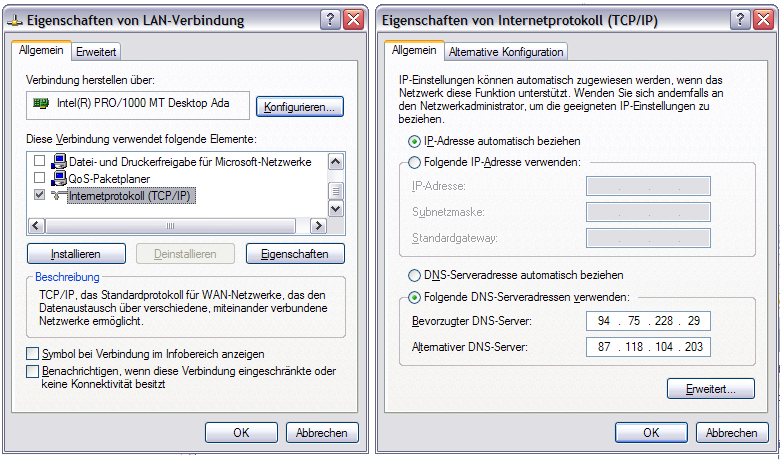
\includegraphics[scale=0.5]{../screenshots/dns_win3.png}
\caption{Konfiguration der DNS-Server (WINDOWS)}
\label{abb:dns1}
\end{center}
\end{figure}

Hier w�hlt man die \textit{TCP-Verbindung} und klickt auf \textit{Eigenschaften}. In dem folgenden Dialog kann man eigene DNS-Server konfigurieren. In dem folgenden Dialog kann man den lokalen bind9 als DNS-Server konfigurieren, indem man als \textit{Bevorzugten DNS-Server} die Adresse \textit{127.0.0.1} eingibt.
